%%%%%%%%%%%%%%%%%%%%%%%%%%%%%%%%%%%%%
%                                   %
% Compile with XeLaTeX and biber    %
%                                   %
% Questions or comments:            %
%                                   %
% joshua dot mcneill at uga dot edu %
%                                   %
%%%%%%%%%%%%%%%%%%%%%%%%%%%%%%%%%%%%%

\documentclass{beamer}
  % Read in standard preamble (cosmetic stuff)
  %%%%%%%%%%%%%%%%%%%%%%%%%%%%%%%%%%%%%%%%%%%%%%%%%%%%%%%%%%%%%%%%
% This is a standard preamble used in for all slide documents. %
% It basically contains cosmetic settings.                     %
%                                                              %
% Joshua McNeill                                               %
% joshua dot mcneill at uga dot edu                            %
%%%%%%%%%%%%%%%%%%%%%%%%%%%%%%%%%%%%%%%%%%%%%%%%%%%%%%%%%%%%%%%%

% Beamer settings
% \usetheme{Berkeley}
\usetheme{CambridgeUS}
% \usecolortheme{dove}
% \usecolortheme{rose}
\usecolortheme{seagull}
\usefonttheme{professionalfonts}
\usefonttheme{serif}
\setbeamertemplate{bibliography item}{}

% Packages and settings
\usepackage{fontspec}
  \setmainfont{Charis SIL}
\usepackage{hyperref}
  \hypersetup{colorlinks=true,
              allcolors=blue}
\usepackage{graphicx}
  \graphicspath{{../../figures/}}
\usepackage[normalem]{ulem}
\usepackage{enumerate}

% Document information
\author{M. McNeill}
\title[FREN2001]{Français 2001}
\institute{\url{joshua.mcneill@uga.edu}}
\date{}

%% Custom commands
% Lexical items
\newcommand{\lexi}[1]{\textit{#1}}
% Gloss
\newcommand{\gloss}[1]{`#1'}
\newcommand{\tinygloss}[1]{{\tiny`#1'}}
% Orthographic representations
\newcommand{\orth}[1]{$\langle$#1$\rangle$}
% Utterances (pragmatics)
\newcommand{\uttr}[1]{`#1'}
% Sentences (pragmatics)
\newcommand{\sent}[1]{\textit{#1}}
% Base dir for definitions
\newcommand{\defs}{../definitions}


  % Packages and settings

  % Document information
  \subtitle[Immeubles et \lexi{choisir}]{Les immeubles et les verbes comme \lexi{choisir}}

\begin{document}
  % Read in the standard intro slides (title page and table of contents)
  \begin{frame}
    \titlepage
    \tiny{Office: % Basically a variable for office hours location
Gilbert 121\\
          Office hours: % Basically a variable for office hours
 lundi, mercredi, vendredi 10:10--11:10
}
  \end{frame}

  \begin{frame}{Les verbes comme \lexi{choisir}}
    \begin{center}
      \begin{tabular}{l | l l | l l}
  \multicolumn{5}{c}{choisir \gloss{to choose}} \\
      & \multicolumn{2}{l |}{singulier} & \multicolumn{2}{l}{pluriel} \\
  \hline
  1re & je         & choisis            & nous        & choisissons \\
  2e  & tu         & choisis            & vous        & choisissez \\
  \hline
  3e  & il (masc)  &                    & ils (masc)  & \\
      & elle (fem) & choisit            & elles (fem) & choisissent \\
      & on         &                    &             & \\
  \hline
  \multicolumn{5}{c}{Impératifs $\to$ choisis, choisissez, choisissons}
\end{tabular}

    \end{center}
    \uncover<2->{
      Quels sont les autres verbes comme \lexi{choisir}?
    }
  \end{frame}

  \begin{frame}{Dans une maison}
    \begin{center}
      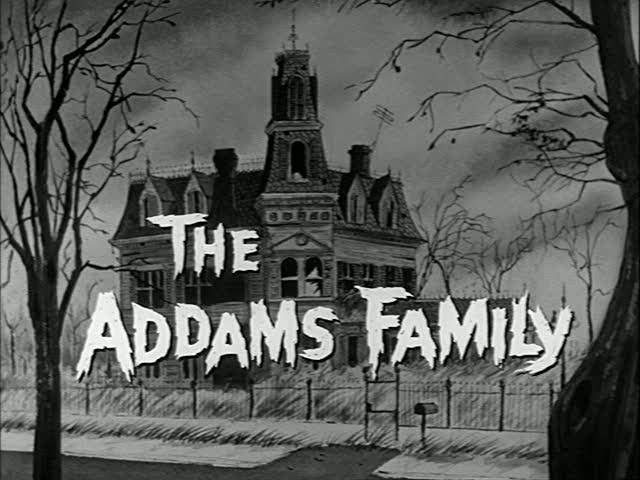
\includegraphics[scale=0.4]{maison_addams.jpg}
    \end{center}
  \end{frame}

  \begin{frame}[t]{Dans une maison}
    \begin{center}
      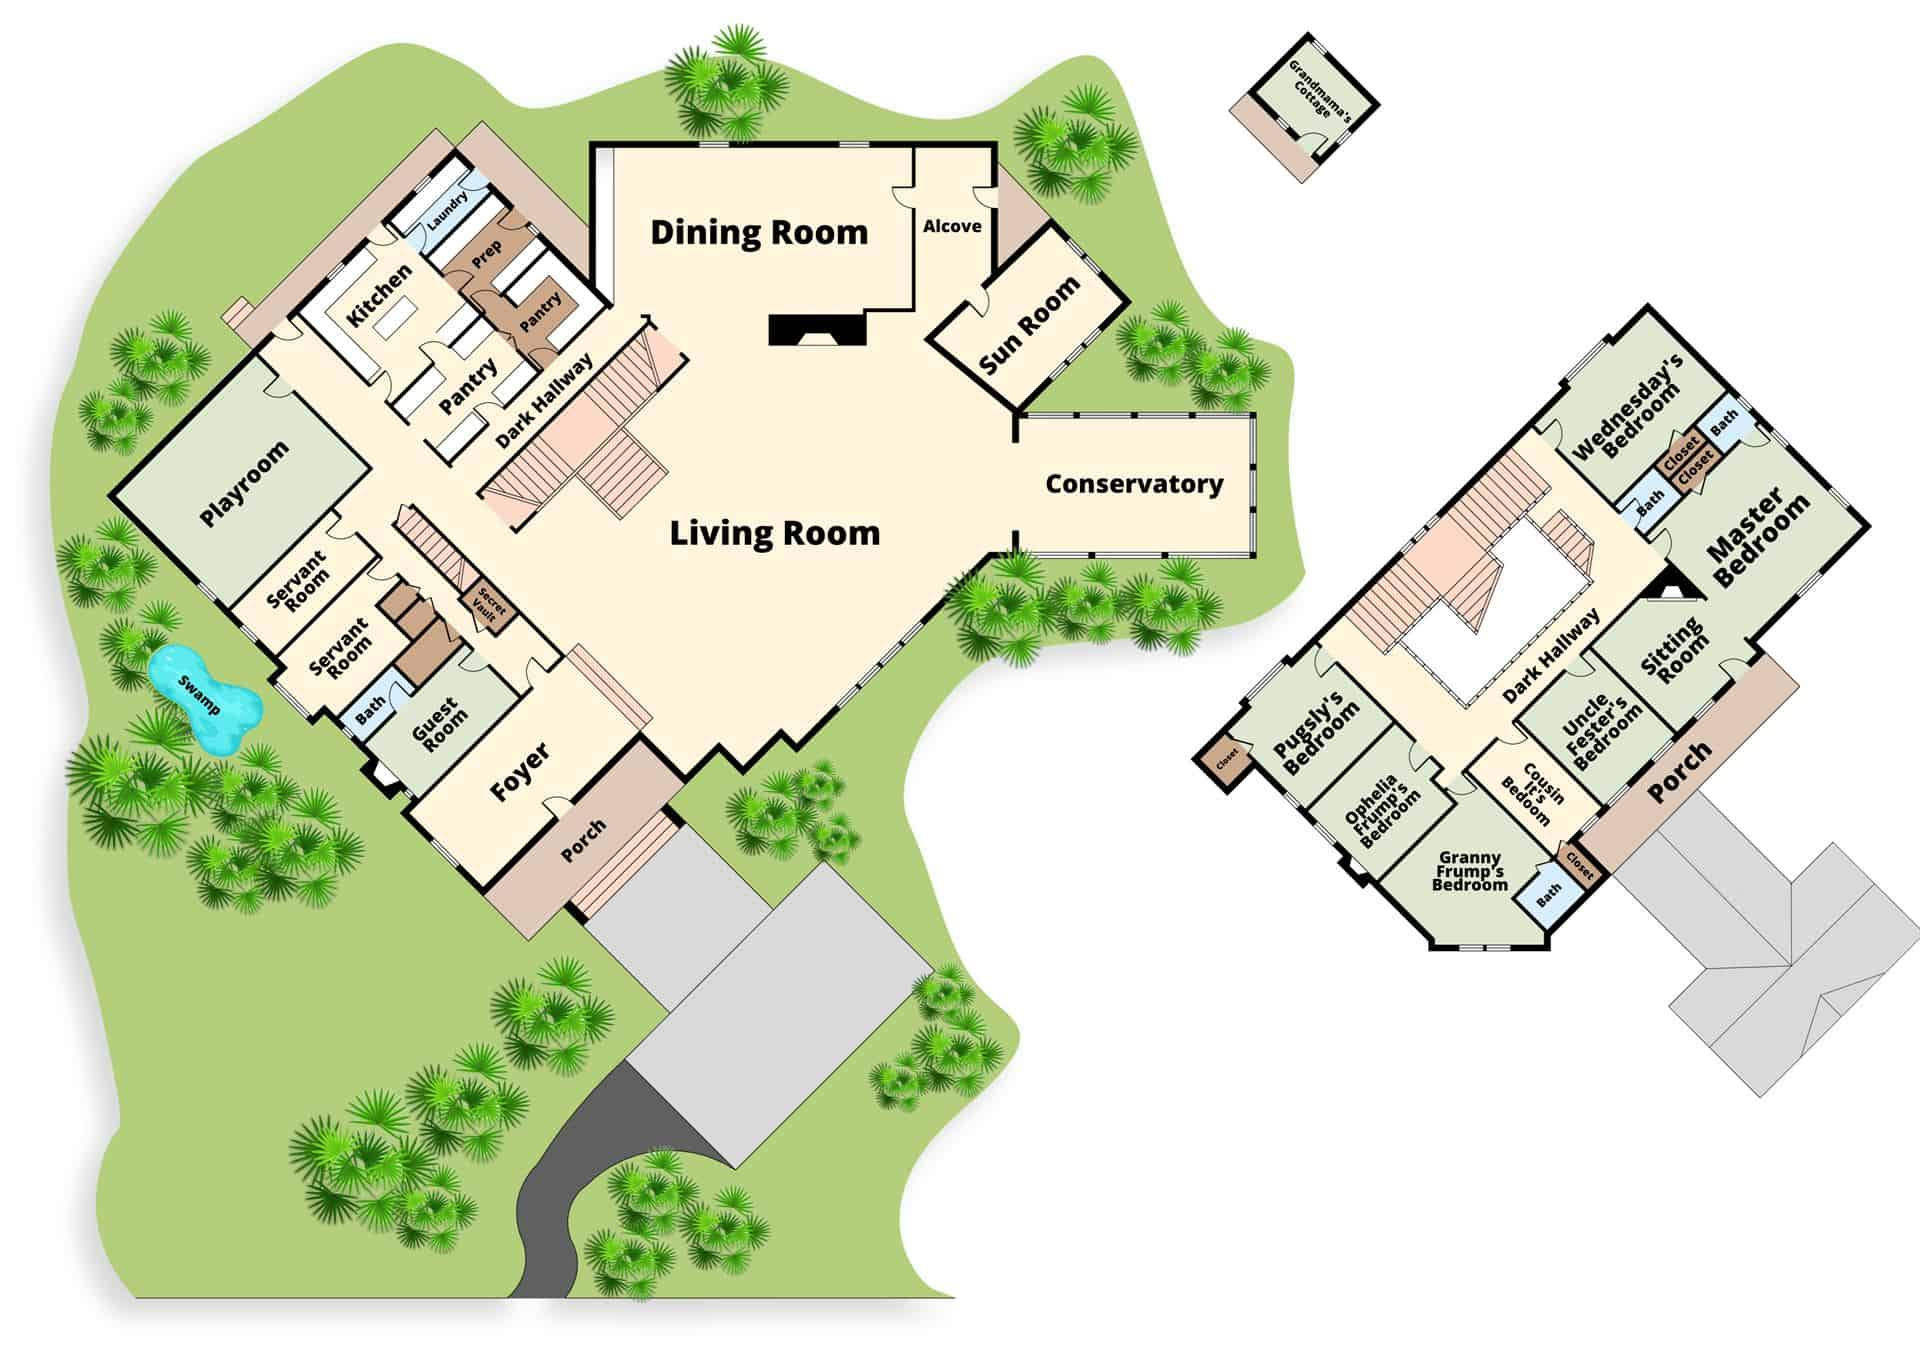
\includegraphics[scale=0.11]{maison_addams_plan.jpg}
    \end{center}
    Où sont ces gens? \\
    \only<1-2>{
      Grandmama prépare le dîner pour la famille. (des grenouilles)\\
      \uncover<2->{$\to$ Elle est dans la cuisine.}
    }
    \only<3-4>{
      Lurch met la table pour les enfants.\\
      \uncover<4->{$\to$ Il est dans la salle à manger.}
    }
    \only<5-6>{
      Gomez prend un bain.\\
      \uncover<6->{$\to$ Il est dans la salle de bains.}
    }
    \only<7-8>{
      Wednesday et Pugsley jouent aux cartes (de tarot).\\
      \uncover<8->{$\to$ Ils sont dans la salle de séjour.}
    }
    \only<9-10>{
      Cousin Itt frappe à la porte.\\
      \uncover<10->{$\to$ Il est dans l'entrée.}
    }
    \only<11-12>{
      Morticia fait la sieste.\\
      \uncover<12->{$\to$ Elle est dans sa chambre.}
    }
    \only<13-14>{
      Thing court entre les salles.\\
      \uncover<14->{$\to$ Il est dans un couloir.}
    }
  \end{frame}

  \begin{frame}{}
    \begin{center}
      \Large Quiz
    \end{center}
  \end{frame}

  \begin{frame}{Trouve une personne}
    Trouve une personne dans la classe qui fait toute chose suivante, puis écris son nom sur un papier.
    N'écris pas un nom plus d'une fois.
    \begin{description}
      \item[\textbf{Modèle:}] \emph{Qui finit toujours ses devoirs avant d'arriver en classe?}
      \item[E1:] Est-ce que tu finis toujours tes devoirs avant d'arriver en classe?
      \item[E2:] Non, je ne finis pas... OR Oui, je finis...
    \end{description}
    \begin{columns}[t]
      \scriptsize
      \column{0.5\textwidth}
        \begin{enumerate}
          \item Qui rougit toujours quand il/elle parle devant un groupe?
          \item Qui finit toujours ses devoirs avant d'arriver en classe?
          \item Qui a fini ses devoirs avant minuit hier soir?
          \item Qui grandit toujours \gloss{still}?
          \item Qui réfléchit toujours avant de répondre?
        \end{enumerate}
      \column{0.5\textwidth}
        \begin{enumerate}
          \setcounter{enumi}{5}
          \item Qui réussit toujours à ses examens?
          \item Qui a réussi au dernier examen de français?
          \item Qui maigrit quand il/elle est stressé/e?
          \item Qui grossit quand il/elle est stressé/e?
          \item Qui n'a jamais désobéi à ses parents?
        \end{enumerate}
    \end{columns}
  \end{frame}

  \begin{frame}{}
    \begin{center}
      \Large Questions?
    \end{center}
  \end{frame}
\end{document}
